% ============================================================
%  Module 6 — Keynes and the Multiplier
%  From Smith to Simulation · University of Edinburgh
% ============================================================
\documentclass[aspectratio=169, 10pt]{beamer}
\usetheme{metropolis}

% --- Edinburgh colours ----------------------------------------
\definecolor{UoERed}{HTML}{7A2318}
\definecolor{UoEGold}{HTML}{B8860B}
\definecolor{CodeBG}{HTML}{F7F3ED}
\definecolor{CodeFrame}{HTML}{D5C9B1}

\setbeamercolor{palette primary}{bg=UoERed, fg=white}
\setbeamercolor{frametitle}{bg=UoERed, fg=white}
\setbeamercolor{title separator}{fg=UoEGold}
\setbeamercolor{progress bar}{fg=UoEGold, bg=UoEGold!20}
\setbeamercolor{alerted text}{fg=UoERed}
\setbeamercolor{block title}{bg=UoERed!15, fg=UoERed}
\setbeamercolor{block body}{bg=UoERed!5}

% --- Packages -------------------------------------------------
\usepackage[T1]{fontenc}
\usepackage{lmodern}
\usepackage{amsmath, amssymb, mathtools}
\usepackage{listings}
\usepackage{graphicx, booktabs}
\usepackage{tikz}
\usetikzlibrary{arrows.meta, positioning, calc, decorations.pathreplacing}
\usepackage{hyperref}
\hypersetup{colorlinks=true, linkcolor=UoERed, urlcolor=UoERed!70!black}
\setbeamertemplate{navigation symbols}{}

\lstset{
  language=Python,
  basicstyle=\ttfamily\scriptsize,
  keywordstyle=\color{UoERed}\bfseries,
  commentstyle=\color{gray}\itshape,
  stringstyle=\color{UoEGold},
  backgroundcolor=\color{CodeBG},
  frame=single,
  rulecolor=\color{CodeFrame},
  numbers=none,
  breaklines=true,
  showstringspaces=false,
  tabsize=4,
  xleftmargin=4pt, xrightmargin=4pt,
  aboveskip=6pt, belowskip=4pt,
}

% Section title pages
\AtBeginSection[]{
  \begin{frame}
    \vfill\centering
    \usebeamerfont{title}\insertsectionhead\par
    \vfill
  \end{frame}
}

% ---- Title ---------------------------------------------------
\title{Module 6 --- Keynes and the Multiplier}
\subtitle{The Great Depression, Aggregate Demand, and Fiscal Policy}
\author{Dr Juan Zurita}
\institute{From Smith to Simulation\\
The University of Edinburgh~$\cdot$~School of Economics}
\date{}

\begin{document}

% =============================================================
\maketitle
% =============================================================

% -------------------------------------------------------------
\section{Part I --- The History}
% -------------------------------------------------------------

\begin{frame}{October 1929: Black Tuesday}
\begin{columns}[T]
\column{0.55\textwidth}
\begin{itemize}
  \item October 29, 1929 --- the New York Stock Exchange crashes.
        Billions of dollars in wealth evaporate within weeks.
  \item What followed was the \textbf{Great Depression}: the most severe
        economic catastrophe of the modern era.
  \item US GDP fell by nearly \alert{30\%} (1929--1933).
  \item Unemployment rose to \alert{25\%}.
  \item World trade collapsed by \alert{two-thirds}.
\end{itemize}
\column{0.4\textwidth}
\begin{block}{The Scale of Disaster}
Factories stood idle. Millions who wanted to work could not find jobs.
And the prevailing economic orthodoxy had no good explanation for
\textit{why} --- and no good prescription for what to do.
\end{block}
\end{columns}
\end{frame}

\begin{frame}{The Classical Orthodoxy: Say's Law}
\begin{block}{Say's Law (1803)}
  ``Supply creates its own demand.''
  \begin{itemize}
    \item A general glut --- an economy-wide shortage of demand ---
          was deemed \textit{impossible}.
    \item If people saved more, interest rates would fall,
          investment would rise, equilibrium would be restored.
    \item The prescription: \textbf{patience}. The market will sort itself out.
  \end{itemize}
\end{block}
\vspace{0.5em}
But as the Depression dragged on year after year, patience began to look
less like wisdom and more like \alert{indifference}.
\end{frame}

\begin{frame}{John Maynard Keynes (1883--1946)}
\begin{columns}[T]
\column{0.55\textwidth}
\begin{itemize}
  \item Cambridge economist, investor, patron of the arts,
        and one of the most brilliant minds of the 20th century.
  \item In \textbf{1936}, he published \textit{The General Theory of
        Employment, Interest, and Money}.
  \item Central argument: \alert{demand matters}.
  \item An economy can get stuck where people want to work but firms
        will not hire, because firms do not expect enough demand.
  \item This is not a temporary glitch --- it can persist \textbf{indefinitely}.
\end{itemize}
\column{0.4\textwidth}
\begin{center}
\textit{``The outstanding faults of the economic society in which we live
are its failure to provide for full employment and its arbitrary and
inequitable distribution of wealth and incomes.''}\\[6pt]
--- Keynes, \textit{General Theory} (1936), Ch.~24
\end{center}
\end{columns}
\end{frame}

\begin{frame}{Key Idea 1: The Paradox of Thrift}
\begin{center}
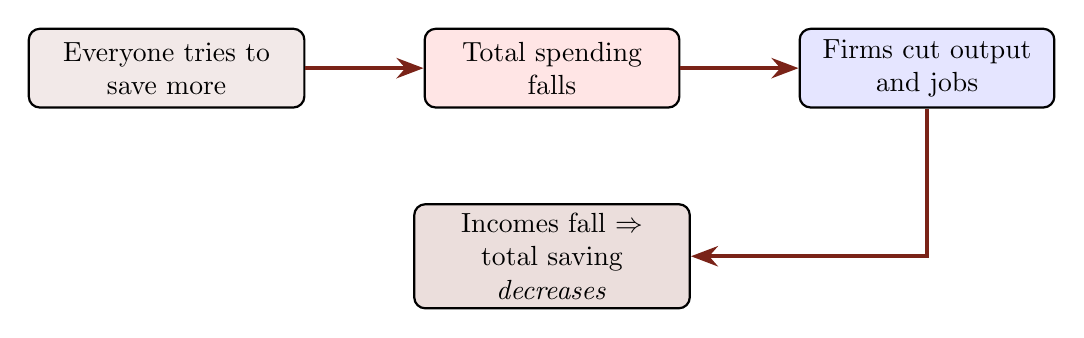
\begin{tikzpicture}[>=Stealth, thick, scale=0.85]
  \node[draw, rounded corners, fill=UoERed!10, minimum width=3.5cm,
        minimum height=1cm, text width=3.2cm, align=center]
    (save) {Everyone tries to\\save more};
  \node[right=1.5cm of save, draw, rounded corners, fill=red!10,
        minimum width=3.2cm, minimum height=1cm, text width=3cm, align=center]
    (spend) {Total spending\\falls};
  \node[right=1.5cm of spend, draw, rounded corners, fill=blue!10,
        minimum width=3.2cm, minimum height=1cm, text width=3cm, align=center]
    (output) {Firms cut output\\and jobs};
  \node[below=1.2cm of spend, draw, rounded corners, fill=UoERed!15,
        minimum width=3.5cm, minimum height=1cm, text width=3.2cm, align=center]
    (result) {Incomes fall $\Rightarrow$\\total saving \textit{decreases}};
  \draw[->, line width=1.5pt, UoERed] (save) -- (spend);
  \draw[->, line width=1.5pt, UoERed] (spend) -- (output);
  \draw[->, line width=1.5pt, UoERed] (output) |- (result);
\end{tikzpicture}
\end{center}
\vspace{0.5em}
What is rational for each individual is \alert{disastrous} for the economy as a whole.\\[4pt]
Smith's invisible hand, which harmonises self-interest and social welfare
in the market for oats, \textbf{breaks down} at the level of the whole economy.
\end{frame}

\begin{frame}{Key Idea 2: Animal Spirits}
\begin{itemize}
  \item Investment depends not just on interest rates (as the classics assumed)
        but on business confidence --- what Keynes called \alert{``animal spirits''}.
  \item When entrepreneurs are optimistic, they invest.
        When they are pessimistic, they do not.
  \item Pessimism can be \textbf{self-fulfilling}: if firms expect a recession,
        they cut investment, which \textit{causes} the recession.
\end{itemize}
\vspace{0.5em}
\begin{alertblock}{A Vicious Circle}
Pessimism $\Rightarrow$ less investment $\Rightarrow$ less output $\Rightarrow$
less income $\Rightarrow$ more pessimism $\Rightarrow$ \ldots
\end{alertblock}
\end{frame}

\begin{frame}{Key Idea 3: The Multiplier}
When the government spends an extra pound:
\vspace{0.3em}
\begin{enumerate}
  \item That pound becomes someone's income.
  \item They spend part of it --- that becomes someone \textit{else's} income.
  \item They spend part of \textit{that} --- and so on.
\end{enumerate}
\vspace{0.3em}
The total effect on GDP is a \textbf{multiple} of the original spending.
\vspace{0.5em}
\[
  \text{Multiplier} = \frac{1}{1 - c_1}
\]
\vspace{0.3em}
where $c_1$ is the \alert{marginal propensity to consume} (MPC) ---
the fraction of each extra pound of income that gets spent.\\[6pt]
With $c_1 = 0.8$: multiplier $= 5$. Every \pounds1 of government spending
generates \pounds5 of output.
\end{frame}

\begin{frame}{The Edinburgh Connection}
\begin{block}{Keynesian Debates at Edinburgh}
Keynes's ideas were fiercely debated in Edinburgh. The University's economics
department in the 1930s and 40s included several economists who were
\textbf{sceptical} of Keynes --- they belonged more to the classical tradition
that Keynes was attacking.
\end{block}
\vspace{0.5em}
This tension between Keynesian macroeconomics and classical market-clearing
models remains alive today, and Edinburgh's department has contributed to
\textbf{both sides} of the argument.
\vspace{0.5em}
\begin{center}
\textit{A university where intellectual disagreement is taken seriously\\
is a university doing its job.}
\end{center}
\end{frame}

% -------------------------------------------------------------
\section{Part II --- The Computation}
% -------------------------------------------------------------

\begin{frame}[fragile]{Setting Up}
\begin{lstlisting}
import numpy as np
import matplotlib.pyplot as plt
from scipy.optimize import fsolve
\end{lstlisting}
\vspace{0.5em}
\begin{itemize}
  \item \texttt{numpy} --- numerical arrays and operations
  \item \texttt{matplotlib} --- plotting
  \item \texttt{fsolve} --- numerical root-finder
        (finds equilibrium by solving $f(x) = 0$)
\end{itemize}
\end{frame}

\begin{frame}{The Keynesian Cross}
The simplest Keynesian model has three sources of spending:
\vspace{0.3em}
\begin{align*}
  C &= c_0 + c_1(Y - T) & &\text{(Consumption)} \\[2pt]
  I &= \bar{I}           & &\text{(Investment --- fixed by animal spirits)} \\[2pt]
  G &= \bar{G}           & &\text{(Government spending --- policy choice)}
\end{align*}
\vspace{0.2em}
\begin{description}
  \item[$c_0$] Autonomous consumption (spending even if income is zero).
  \item[$c_1$] \textbf{MPC}: fraction of each extra pound of disposable income spent.
  \item[$Y - T$] Disposable income (income minus taxes).
\end{description}
\vspace{0.3em}
\textbf{Equilibrium:} output $=$ total spending:
\[
  Y = C + I + G = c_0 + c_1(Y - T) + \bar{I} + G
\]
\end{frame}

\begin{frame}[fragile]{Defining the Model in Python}
\begin{lstlisting}
# Parameters
c0 = 100    # autonomous consumption
c1 = 0.6    # marginal propensity to consume (MPC)
I_bar = 200 # investment (animal spirits)
G = 150     # government spending
T = 100     # taxes

def consumption(Y, c0=c0, c1=c1, T=T):
    return c0 + c1 * (Y - T)

def total_spending(Y, c0=c0, c1=c1, I_bar=I_bar, G=G, T=T):
    return consumption(Y, c0, c1, T) + I_bar + G

def equilibrium_condition(Y, c0=c0, c1=c1, I_bar=I_bar, G=G, T=T):
    """Returns zero when Y = C + I + G."""
    return Y - total_spending(Y, c0, c1, I_bar, G, T)
\end{lstlisting}
\end{frame}

\begin{frame}[fragile]{Finding Equilibrium with \texttt{fsolve}}
\textbf{Analytical} (for the linear model):
\[
  Y^* = \frac{c_0 - c_1 T + \bar{I} + G}{1 - c_1}
     = \frac{100 - 60 + 200 + 150}{0.4} = \frac{390}{0.4} = 975
\]

\textbf{Numerical} (works for \textit{any} specification):
\begin{lstlisting}
Y_star = fsolve(equilibrium_condition, x0=500)[0]
C_star = consumption(Y_star)

print(f"Y* = {Y_star:.2f}")   # 975.00
print(f"C* = {C_star:.2f}")   # 625.00
print(f"C + I + G = {C_star + I_bar + G:.2f}")  # 975.00
\end{lstlisting}
\vspace{0.3em}
Numerical and analytical solutions agree to machine precision.
\end{frame}

\begin{frame}{Visualising the Keynesian Cross}
\begin{center}
\begin{tikzpicture}[scale=0.55, >=Stealth]
  % Axes
  \draw[->] (0,0) -- (11,0) node[below] {$Y$};
  \draw[->] (0,0) -- (0,11) node[left] {Spending};
  % 45-degree line
  \draw[dashed, black, thin] (0,0) -- (10.5,10.5);
  \node[above, font=\scriptsize, rotate=45] at (9.5,9.8) {$45^{\circ}$};
  % Spending line: E = c0 + c1(Y-T) + I + G
  % E = 100 + 0.6*(Y-100) + 200 + 150 = 390 + 0.6*Y
  % At Y=0: E=390; at Y=975: E=975
  % Scale: Y in [0,1800] mapped to [0,10]; E same
  % Y=0 -> x=0, E=390 -> y=390/180=2.17
  % Y=975 -> x=975/180=5.42, E=975 -> y=5.42
  % Y=1800 -> x=10, E=390+0.6*1800=1470 -> y=8.17
  \draw[thick, blue] (0, 2.17) -- (10, 8.17)
    node[right, font=\small] {$C+I+G$};
  % Equilibrium
  \filldraw[red] (5.42, 5.42) circle (3pt);
  \draw[dashed, gray] (5.42, 0) -- (5.42, 5.42) -- (0, 5.42);
  \node[below, font=\scriptsize] at (5.42, 0) {$Y^{*}\!=\!975$};
  \node[left, font=\scriptsize] at (0, 5.42) {$975$};
  % Autonomous spending label
  \draw[dotted, gray] (0, 2.17) -- (1.5, 2.17);
  \node[right, font=\scriptsize, gray] at (1.5, 2.17) {$390$};
\end{tikzpicture}
\end{center}
\vspace{0.3em}
Equilibrium is where the spending line crosses the $45^{\circ}$ line:
output equals planned spending.
\end{frame}

\begin{frame}{The Fiscal Multiplier}
What happens when the government increases spending by $\Delta G$?
\vspace{0.3em}
\[
  Y^* = \frac{c_0 - c_1 T + \bar{I} + G}{1 - c_1}
  \quad\Longrightarrow\quad
  \frac{\Delta Y}{\Delta G} = \frac{1}{1 - c_1}
\]
\vspace{0.3em}
\begin{columns}[T]
\column{0.48\textwidth}
\begin{block}{With $c_1 = 0.6$}
  Multiplier $= \dfrac{1}{1 - 0.6} = 2.5$\\[6pt]
  Every \pounds1 spent $\Rightarrow$ \pounds2.50 of output.
\end{block}
\column{0.48\textwidth}
\begin{block}{With $c_1 = 0.8$}
  Multiplier $= \dfrac{1}{1 - 0.8} = 5.0$\\[6pt]
  Every \pounds1 spent $\Rightarrow$ \pounds5.00 of output.
\end{block}
\end{columns}
\vspace{0.5em}
The MPC $c_1$ is the \textbf{engine} of the multiplier.
Higher MPC $\Rightarrow$ larger multiplier $\Rightarrow$ more potent fiscal policy.
\end{frame}

\begin{frame}[fragile]{Computing the Multiplier}
\begin{lstlisting}
delta_G = 50
G_new = G + delta_G

Y_star_new = fsolve(equilibrium_condition, x0=500,
                    args=(c0, c1, I_bar, G_new, T))[0]

delta_Y = Y_star_new - Y_star
multiplier_numerical = delta_Y / delta_G
multiplier_theory = 1 / (1 - c1)

print(f"Original Y*: {Y_star:.2f}")      # 975.00
print(f"New Y*:      {Y_star_new:.2f}")   # 1100.00
print(f"Delta Y:     {delta_Y:.2f}")      # 125.00
print(f"Numerical multiplier:   {multiplier_numerical:.4f}")
print(f"Theoretical multiplier: {multiplier_theory:.4f}")
# Both equal 2.5000
\end{lstlisting}
\end{frame}

\begin{frame}{The Multiplier Round by Round}
Trace how a $\Delta G = 50$ ripples through the economy:
\vspace{0.3em}
\begin{center}
\begin{tabular}{clr@{\qquad}r}
\toprule
\textbf{Round} & \textbf{Who earns?} & \textbf{New spending} & \textbf{Cumulative} \\
\midrule
1 & Road builders     & $50.00$  & $50.00$ \\
2 & Shopkeepers       & $30.00$  & $80.00$ \\
3 & Suppliers         & $18.00$  & $98.00$ \\
4 & Their suppliers   & $10.80$  & $108.80$ \\
5 & \ldots            & $\;6.48$ & $115.28$ \\
\midrule
$\infty$ & & $0$ & $\mathbf{125.00}$ \\
\bottomrule
\end{tabular}
\end{center}
\vspace{0.3em}
\[
  \Delta G + \Delta G \cdot c_1 + \Delta G \cdot c_1^2 + \cdots
  = \frac{\Delta G}{1 - c_1} = \frac{50}{0.4} = 125
\]
A geometric series --- each round smaller, but they \textbf{add up}.
\end{frame}

\begin{frame}[fragile]{Visualising the Multiplier Process}
\begin{lstlisting}
n_rounds = 20
spending_per_round = [delta_G * c1**r for r in range(n_rounds)]
cumulative = np.cumsum(spending_per_round)

fig, axes = plt.subplots(1, 2, figsize=(12, 4.5))
axes[0].bar(range(1, n_rounds+1), spending_per_round,
            color='steelblue', alpha=0.7)
axes[0].set_xlabel('Round'); axes[0].set_ylabel('New spending')
axes[0].set_title('Spending per Round')

axes[1].plot(range(1, n_rounds+1), cumulative, 'o-', color='coral')
axes[1].axhline(delta_G/(1-c1), color='k', linestyle='--',
                label=f'Limit = {delta_G/(1-c1):.0f}')
axes[1].set_xlabel('Round')
axes[1].set_title('Cumulative Multiplier Effect')
axes[1].legend()
plt.tight_layout(); plt.show()
\end{lstlisting}
\end{frame}

\begin{frame}{Cumulative Multiplier: Convergence}
\begin{center}
\begin{tikzpicture}[scale=0.65, >=Stealth]
  % Axes
  \draw[->] (0,0) -- (11,0) node[below] {Round};
  \draw[->] (0,0) -- (0,7) node[left] {\pounds};
  % Limit line at 125 => y=6
  \draw[dashed, black] (0, 6) -- (10.5, 6);
  \node[left, font=\scriptsize] at (0, 6) {$125$};
  % Cumulative curve (scaled: 125 -> 6)
  % Round 1: 50 => 2.4, Round 2: 80 => 3.84, Round 3: 98 => 4.70
  % Round 4: 108.8 => 5.22, Round 5: 115.28 => 5.53
  % Round 6: 119.17 => 5.72, Round 7: 121.50 => 5.83
  % Round 8: 122.90 => 5.90, Round 9: 123.74 => 5.94
  % Round 10: 124.24 => 5.96
  \draw[thick, red] plot[smooth, mark=*, mark size=2pt] coordinates
    {(1,2.4) (2,3.84) (3,4.70) (4,5.22) (5,5.53)
     (6,5.72) (7,5.83) (8,5.90) (9,5.94) (10,5.96)};
  % Labels
  \node[right, font=\scriptsize] at (10.5, 6) {$\frac{\Delta G}{1-c_1}$};
  \node[below, font=\scriptsize] at (1,0) {1};
  \node[below, font=\scriptsize] at (5,0) {5};
  \node[below, font=\scriptsize] at (10,0) {10};
\end{tikzpicture}
\end{center}
\vspace{0.3em}
The cumulative effect converges quickly to the theoretical multiplier.
After 10~rounds, we have captured 98\% of the total effect.
\end{frame}

\begin{frame}[fragile]{How the MPC Changes the Multiplier}
\begin{lstlisting}
c1_values = np.linspace(0.1, 0.95, 200)
multipliers = 1 / (1 - c1_values)

fig, ax = plt.subplots(figsize=(8, 5))
ax.plot(c1_values, multipliers, color='steelblue', linewidth=2.5)

for c1_mark, name in [(0.5, 'Cautious'), (0.6, 'Moderate'),
                       (0.8, 'Confident'), (0.9, 'Exuberant')]:
    m = 1 / (1 - c1_mark)
    ax.plot(c1_mark, m, 'o', markersize=8)
    ax.annotate(f'{name}\nc1={c1_mark}, m={m:.1f}',
                xy=(c1_mark, m), xytext=(c1_mark-0.08, m+1.5),
                fontsize=9, ha='center')
ax.set_xlabel('MPC'); ax.set_ylabel('Multiplier = 1/(1-c1)')
ax.set_title('The Multiplier Depends on How Much People Spend')
plt.show()
\end{lstlisting}
\vspace{0.3em}
As $c_1 \to 1$ the multiplier explodes; as $c_1 \to 0$ it shrinks to 1.
\end{frame}

\begin{frame}{MPC Sensitivity: Intuition}
\begin{center}
\begin{tikzpicture}[scale=0.6, >=Stealth]
  \draw[->] (0,0) -- (11,0) node[below] {MPC ($c_1$)};
  \draw[->] (0,0) -- (0,9) node[left] {Multiplier};
  % Plot approximate curve: m = 1/(1-c1), c1 in [0.1, 0.95]
  % c1=0.1 -> m=1.11, c1=0.3 -> 1.43, c1=0.5 -> 2, c1=0.6 -> 2.5
  % c1=0.7 -> 3.33, c1=0.8 -> 5, c1=0.9 -> 10
  % x-scale: c1 in [0,1] -> [0,10]; y-scale: m in [0,12] -> [0,8]
  \draw[thick, blue] plot[smooth] coordinates
    {(1,0.74) (2,0.87) (3,0.95) (4,1.11) (5,1.33)
     (6,1.67) (7,2.22) (8,3.33) (9,6.67)};
  % Markers
  \foreach \cx/\cy/\lab in {5/1.33/Cautious, 6/1.67/Moderate, 8/3.33/Confident, 9/6.67/Exuberant}{
    \filldraw[red] (\cx, \cy) circle (3pt);
    \node[above right, font=\scriptsize] at (\cx, \cy) {\lab};
  }
  % Axis labels
  \node[below, font=\scriptsize] at (1,0) {0.1};
  \node[below, font=\scriptsize] at (5,0) {0.5};
  \node[below, font=\scriptsize] at (8,0) {0.8};
  \node[below, font=\scriptsize] at (9,0) {0.9};
  \node[left, font=\scriptsize] at (0,1.33) {2};
  \node[left, font=\scriptsize] at (0,3.33) {5};
  \node[left, font=\scriptsize] at (0,6.67) {10};
\end{tikzpicture}
\end{center}
\vspace{0.3em}
\textit{``The MPC is the crucial behavioural parameter.''} --- Keynes.\\[4pt]
Economies where people spend more of each extra pound see
\textbf{larger multiplier effects} from government spending.
\end{frame}

\begin{frame}{The IS Curve: Adding Interest Rates}
In the real economy, investment responds to the interest rate $r$:
\[
  I(r) = \bar{I} - d \cdot r
\]
where $d$ measures investment sensitivity to the interest rate.
\vspace{0.5em}

Equilibrium now depends on $r$. For each interest rate, there is a
different equilibrium output $Y^*$.
\vspace{0.3em}
\[
  Y = c_0 + c_1(Y - T) + (\bar{I} - d\,r) + G
\]
\vspace{0.3em}
The set of all $(Y, r)$ pairs where the goods market is in equilibrium
is the \alert{IS curve} (``Investment $=$ Saving'').
\end{frame}

\begin{frame}[fragile]{Computing the IS Curve}
\begin{lstlisting}
d = 500  # investment sensitivity to interest rate

def investment(r, I_bar=200, d=500):
    return I_bar - d * r

def is_equation(Y, r, c0=100, c1=0.6, I_bar=200, d=500,
                G=150, T=100):
    C = c0 + c1 * (Y - T)
    I = I_bar - d * r
    return Y - C - I - G

# For each r, find equilibrium Y
r_values = np.linspace(0.01, 0.15, 50)
Y_is = np.array([fsolve(is_equation, x0=500, args=(r,))[0]
                  for r in r_values])

fig, ax = plt.subplots(figsize=(8, 5))
ax.plot(Y_is, r_values * 100, color='steelblue', linewidth=2.5)
ax.set_xlabel('Output (Y)'); ax.set_ylabel('Interest rate (%)')
ax.set_title('The IS Curve')
ax.set_ylim(16, 0)
plt.show()
\end{lstlisting}
\end{frame}

\begin{frame}{The IS Curve: Graphical View}
\begin{center}
\begin{tikzpicture}[scale=0.65, >=Stealth]
  \draw[->] (0,0) -- (11,0) node[below] {$Y$};
  \draw[->] (0,0) -- (0,8) node[left] {$r$ (\%)};
  % IS curve: Y* = (c0 - c1*T + I_bar - d*r + G)/(1-c1)
  % = (100-60+200-500r+150)/0.4 = (390-500r)/0.4 = 975-1250r
  % At r=0.01 (1%): Y=962.5; at r=0.15 (15%): Y=787.5
  % Scale: Y in [600, 1100] -> x in [0,10]; r in [0,16%] -> y in [0,8]
  % r=1% -> y=0.5; r=15% -> y=7.5
  % Y=962.5 -> x=(962.5-600)/50=7.25; Y=787.5 -> x=(787.5-600)/50=3.75
  \draw[thick, blue] (7.25, 0.5) -- (3.75, 7.5)
    node[above left, font=\small] {IS};
  % Arrow showing slope
  \node[right, font=\scriptsize, text width=3.5cm] at (7.5, 4)
    {Lower $r$ $\Rightarrow$ more investment\\$\Rightarrow$ higher $Y^*$};
  % Axis labels
  \node[below, font=\scriptsize] at (3.75, 0) {$788$};
  \node[below, font=\scriptsize] at (7.25, 0) {$963$};
  \node[left, font=\scriptsize] at (0, 0.5) {$1$};
  \node[left, font=\scriptsize] at (0, 7.5) {$15$};
\end{tikzpicture}
\end{center}
\vspace{0.3em}
The IS curve slopes \textbf{downward}: lower $r$ $\Rightarrow$ cheaper borrowing
$\Rightarrow$ more investment $\Rightarrow$ higher equilibrium output.
\end{frame}

\begin{frame}[fragile]{Fiscal Policy Shifts the IS Curve}
\begin{lstlisting}
fig, ax = plt.subplots(figsize=(8, 5))

for G_val, color, label in [
        (150, 'steelblue', 'G = 150 (original)'),
        (200, 'coral',     'G = 200 (expansion)'),
        (100, 'seagreen',  'G = 100 (austerity)')]:
    Y_is_shift = np.array([
        fsolve(is_equation, x0=500,
               args=(r, c0, c1, I_bar, d, G_val, T))[0]
        for r in r_values])
    ax.plot(Y_is_shift, r_values*100, color=color,
            linewidth=2, label=label)

ax.set_xlabel('Output (Y)'); ax.set_ylabel('Interest rate (%)')
ax.set_title('Fiscal Policy Shifts the IS Curve')
ax.legend(); ax.set_ylim(16, 0)
plt.show()
\end{lstlisting}
\vspace{0.3em}
Keynes's prescription: shift the IS curve \textbf{right} by increasing $G$.
\end{frame}

\begin{frame}{IS Shifts: The Graphical Argument}
\begin{center}
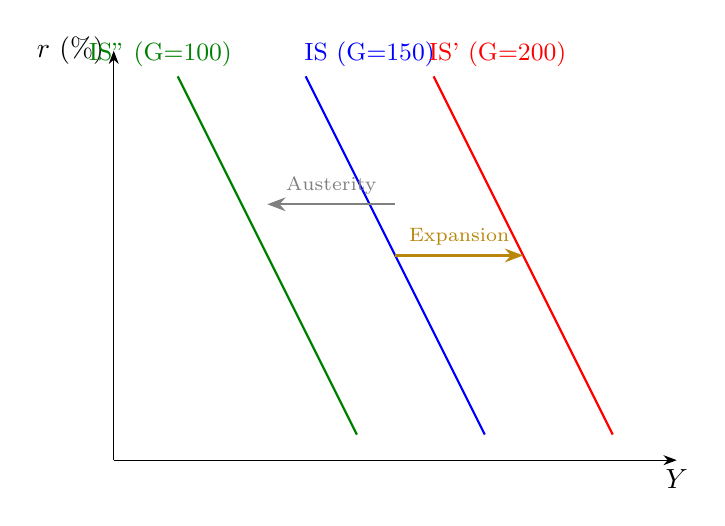
\begin{tikzpicture}[scale=0.65, >=Stealth]
  \draw[->] (0,0) -- (11,0) node[below] {$Y$};
  \draw[->] (0,0) -- (0,8) node[left] {$r$ (\%)};
  % Original IS: Y = 975 - 1250r
  \draw[thick, blue] (7.25, 0.5) -- (3.75, 7.5);
  \node[above, font=\small, blue] at (5.0, 7.5) {IS (G=150)};
  % Expansion IS: Y = (390-60+50)/0.4 - 1250r = 1100 - 1250r (wait, let me recalc)
  % G=200: Y = (100-60+200-500r+200)/0.4 = (440-500r)/0.4 = 1100-1250r
  % r=0.01: Y=1087.5 -> x=(1087.5-600)/50=9.75; r=0.15: Y=912.5 -> x=6.25
  \draw[thick, red] (9.75, 0.5) -- (6.25, 7.5);
  \node[above, font=\small, red] at (7.5, 7.5) {IS' (G=200)};
  % Austerity IS: G=100: Y = (100-60+200-500r+100)/0.4 = (340-500r)/0.4 = 850-1250r
  % r=0.01: Y=837.5 -> x=4.75; r=0.15: Y=662.5 -> x=1.25
  \draw[thick, green!50!black] (4.75, 0.5) -- (1.25, 7.5);
  \node[above left, font=\small, green!50!black] at (2.5, 7.5) {IS'' (G=100)};
  % Arrows
  \draw[->, thick, UoEGold] (5.5, 4) -- (8.0, 4)
    node[midway, above, font=\scriptsize] {Expansion};
  \draw[->, thick, gray] (5.5, 5) -- (3.0, 5)
    node[midway, above, font=\scriptsize] {Austerity};
\end{tikzpicture}
\end{center}
\vspace{0.3em}
At every interest rate, higher $G$ means higher equilibrium output.\\
The government spends what the private sector will not.
\end{frame}

\begin{frame}{Animal Spirits: Confidence Crash Simulation}
\begin{columns}[T]
\column{0.55\textwidth}
Simulate 40~quarters:
\begin{itemize}
  \item Quarters 1--10: $\bar{I} = 200$ (normal confidence).
  \item Quarter 10: confidence crashes $\Rightarrow$ $\bar{I} = 140$.
  \item \textbf{Scenario A:} No policy response.
  \item \textbf{Scenario B:} Government raises $G$ by 40
        two quarters later (quarter 12).
\end{itemize}
\column{0.4\textwidth}
\begin{center}
\begin{tikzpicture}[scale=0.45, >=Stealth]
  \draw[->] (0,0) -- (9,0) node[below, font=\scriptsize] {Quarter};
  \draw[->] (0,0) -- (0,6) node[left, font=\scriptsize] {$\bar{I}$};
  \draw[thick, red] (0,4.5) -- (2.5,4.5) -- (2.5,2.5) -- (8,2.5);
  \draw[dashed, gray] (2.5,0) -- (2.5,4.5);
  \node[below, font=\tiny] at (2.5,0) {$t\!=\!10$};
  \node[left, font=\tiny] at (0,4.5) {$200$};
  \node[left, font=\tiny] at (0,2.5) {$140$};
  \node[above, font=\tiny, red] at (5, 2.7) {Crash};
\end{tikzpicture}
\end{center}
\end{columns}
\end{frame}

\begin{frame}[fragile]{Animal Spirits: Python Simulation}
\begin{lstlisting}
T_sim = 40; r_fixed = 0.05
I_bar_path = np.ones(T_sim) * 200
I_bar_path[10:] = 140  # confidence crash at quarter 10

Y_path = np.array([
    fsolve(is_equation, 500,
           args=(r_fixed, c0, c1, I_bar_path[t], d, G, T))[0]
    for t in range(T_sim)])

# With fiscal response: G increases by 40 at quarter 12
G_resp = np.ones(T_sim) * G
G_resp[12:] = G + 40

Y_path_resp = np.array([
    fsolve(is_equation, 500,
           args=(r_fixed, c0, c1, I_bar_path[t], d, G_resp[t], T))[0]
    for t in range(T_sim)])

print(f"Drop without intervention: {Y_path[0]-Y_path[15]:.0f}")
print(f"Drop with fiscal stimulus: {Y_path[0]-Y_path_resp[15]:.0f}")
\end{lstlisting}
\end{frame}

\begin{frame}{Keynes vs.\ Doing Nothing}
\begin{center}
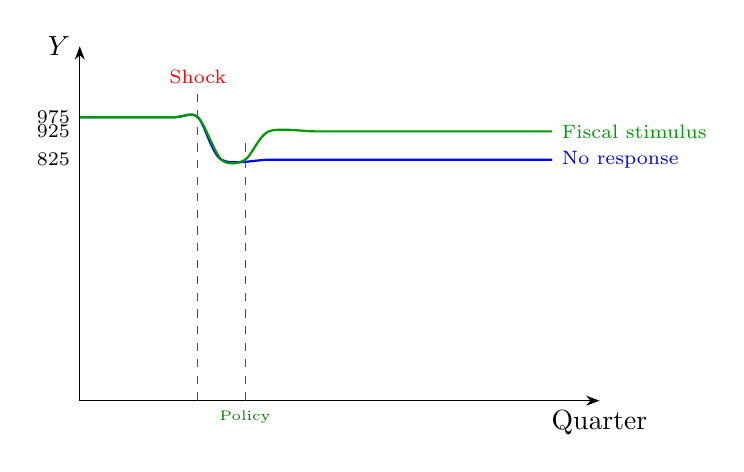
\begin{tikzpicture}[scale=0.6, >=Stealth]
  \draw[->] (0,0) -- (11,0) node[below] {Quarter};
  \draw[->] (0,0) -- (0,7.5) node[left] {$Y$};
  % Y_pre = 975 (say y=6), Y_post_nopol = 975-150=825 (y~=5.1)
  % Y_post_pol = 825+100=925 (y~=5.7) [G+40, mult 2.5 => delta_Y=100]
  % No policy
  \draw[thick, blue] plot[smooth, mark=none] coordinates
    {(0,6) (1,6) (2,6) (2.5,6)
     (3,5.1) (4,5.1) (5,5.1) (6,5.1) (7,5.1) (8,5.1) (9,5.1) (10,5.1)};
  \node[right, font=\scriptsize, blue] at (10, 5.1) {No response};
  % With policy
  \draw[thick, green!60!black] plot[smooth, mark=none] coordinates
    {(0,6) (1,6) (2,6) (2.5,6)
     (3,5.1) (3.5,5.1) (4,5.7) (5,5.7) (6,5.7) (7,5.7) (8,5.7) (9,5.7) (10,5.7)};
  \node[right, font=\scriptsize, green!60!black] at (10, 5.7) {Fiscal stimulus};
  % Shock line
  \draw[dashed, red, thin] (2.5, 0) -- (2.5, 6.5);
  \node[above, font=\scriptsize, red] at (2.5, 6.5) {Shock};
  \draw[dashed, green!50!black, thin] (3.5, 0) -- (3.5, 5.5);
  \node[below, font=\tiny, green!50!black] at (3.5, 0) {Policy};
  % Y labels
  \node[left, font=\scriptsize] at (0, 6) {$975$};
  \node[left, font=\scriptsize] at (0, 5.1) {$825$};
  \node[left, font=\scriptsize] at (0, 5.7) {$925$};
\end{tikzpicture}
\end{center}
\vspace{0.3em}
Government spending \textbf{partially offsets} the confidence crash.\\[4pt]
\textit{``When animal spirits fail, the government must step in
to maintain demand.''} --- Keynes's core policy argument.
\end{frame}

% -------------------------------------------------------------
\section{Part III --- Exercises \& Discussion}
% -------------------------------------------------------------

\begin{frame}{Exercise 1: The Paradox of Thrift}
Starting from the baseline ($c_0 = 100$, $c_1 = 0.6$, $\bar{I} = 200$,
$G = 150$, $T = 100$):
\vspace{0.3em}
\begin{enumerate}
  \item Compute equilibrium $Y^*$ for $c_1 = 0.6,\ 0.5,\ 0.4,\ 0.3$.\\
        Show that output \textit{falls} as people save more.
  \item Compute total saving $S = Y - C - T$ at each equilibrium.\\
        Does saving actually \textit{increase} when people try to save more?
  \item Plot $Y^*$ and $S$ against $c_1$. This is the paradox of thrift in action.
  \item In 2--3 sentences: why is what is rational for each individual
        harmful for the economy as a whole?
        How does this relate to Smith's invisible hand?
\end{enumerate}
\end{frame}

\begin{frame}{Exercise 2: The Balanced-Budget Multiplier}
A politician proposes increasing $G$ by \pounds100, financed entirely
by a \pounds100 tax increase ($\Delta G = \Delta T = 100$).
\vspace{0.3em}
\begin{enumerate}
  \item Compute $Y^*$ with $G = 150$, $T = 100$ (baseline).
  \item Compute $Y^*$ with $G = 250$, $T = 200$ (balanced-budget expansion).
  \item What is $\Delta Y$? Is the balanced-budget multiplier
        equal to $0$, $1$, or something else?
  \item Explain intuitively why a balanced-budget expansion still
        increases output.
\end{enumerate}
\vspace{0.5em}
\begin{alertblock}{Hint}
The government spends 100\% of the extra revenue, but taxpayers
only reduce their spending by $c_1 \times 100$.
The net injection is $(1 - c_1) \times 100$.
\end{alertblock}
\end{frame}

\begin{frame}{Exercise 3: Progressive Tax as Automatic Stabiliser}
Replace the lump-sum tax $T$ with a \textbf{proportional income tax}:
$T(Y) = \tau \cdot Y$.
\vspace{0.3em}

The consumption function becomes:
\[
  C = c_0 + c_1\,(1 - \tau)\,Y
\]

\begin{enumerate}
  \item Write a new equilibrium condition. Use $\tau = 0.25$.
  \item Find $Y^*$ with \texttt{fsolve}. Compare to the fixed-tax model.
  \item Derive the new multiplier formula:
  \[
    \text{Multiplier} = \frac{1}{1 - c_1(1 - \tau)}
  \]
  Verify numerically by increasing $G$ by $50$.
  \item Compare multipliers for $\tau = 0$, $0.25$, $0.5$.\\
        Keynes's followers called the income tax an \alert{automatic stabiliser} ---
        explain why.
\end{enumerate}
\end{frame}

% -------------------------------------------------------------
\section{Key Takeaways}
% -------------------------------------------------------------

\begin{frame}{What We Learned This Week}
\begin{enumerate}
  \item The \textbf{Great Depression} (1929--33) shattered the classical belief
        that markets always self-correct.
  \item Keynes (1936) argued that \alert{aggregate demand} can be persistently
        deficient --- economies can get stuck below full employment.
  \item The \textbf{consumption function} $C = c_0 + c_1(Y-T)$ and the
        \textbf{Keynesian cross} provide a tractable model of output
        determination.
  \item The \textbf{fiscal multiplier} $1/(1-c_1)$ shows that government
        spending has amplified effects on output.
  \item The \textbf{IS curve} links interest rates to equilibrium output
        and illustrates how fiscal policy shifts aggregate demand.
  \item \textbf{Animal spirits} can cause self-fulfilling recessions;
        fiscal policy can partially offset confidence collapses.
\end{enumerate}
\end{frame}

\begin{frame}{Further Reading}
\begin{itemize}
  \item Keynes, J.M. \textit{The General Theory of Employment, Interest, and
        Money} (1936), Chs.~1--3, 10 (the multiplier).
  \item Skidelsky, R. \textit{Keynes: A Very Short Introduction} ---
        an excellent 150-page overview.
  \item Heilbroner, R. \textit{The Worldly Philosophers}, Ch.~9
        (``The Heresies of John Maynard Keynes'').
  \item Hicks, J.R. ``Mr.\ Keynes and the `Classics'\,'' (1937) ---
        the paper that invented the IS-LM model.
\end{itemize}
\vspace{1em}
\begin{center}
\textbf{Next week:} Marx and the Machinery Question ---\\
capital accumulation, the labour share of income,\\
and the debate over whether technology helps or hurts workers.
\end{center}
\end{frame}

\end{document}
